\section{Energy Detection with Perfect Side Information}
\subsection{System Model}
We consider a cognitive radio system where the licensed frequency spectrum could be occupied by one of two distinct signals $\{s_A, s_B\}$ or it could be vacant. 
Assume the detector has perfect side information of primary users, i.e. for a specific time slot the detector knows which primary user could occupy the channel. For easy presentation, let $T_A$ presents the time slot during which the channel can be either ideal or occupied by primary signal $s_A$. Let $T_B$ denote the time slot during which the channel can be either ideal or occupied by primary signal $s_B$. We can see, during time slot $T_A$, primary user $s_B$ will not present in the channel and during time slot $T_B$ primary user $s_A$ will not present in the channel. Since the detector has perfect side information, it knows the beginnings and endings for $T_A$ and $T_B$. Let $H_0$ denote the hypothesis under which the channel is free,  $H_1$ denote the hypothesis under which the channel is occupied by $s_A$ and $H_2$ denote the hypothesis under which the channel is occupied by $s_B$, i.e.
\begin{equation}
\begin{cases}
H_0:\;\;\;\;\text{channel is free}\\
H_1:\;\;\;\;\text{channel is occupied by $s_A$}\\
H_2:\;\;\;\;\text{channel is occupied by $s_B$}\,.
\end{cases}
\end{equation} 

During time slot $T_A$, we  test $H_0$ against $H_1$; during time slot $T_B$, we test $H_0$ against $H_2$. 
Even though there are three hypotheses, for a specific time slot, it is still a two hypotheses testing problem.  
For both $T_A$ and $T_B$, we use energy detector to decide the status of the channel. Let $\mathbf{x}$ denote the input of the detector, $Y$ denote the testing statistics of the received signal (in this case, $Y$ is the energy of the sampled signal), $n$  denote the system noise and $s_A$ ($s_B$) denote the transmitted signal, thus we have
\begin{eqnarray}
  \mathbf{x} = \begin{cases}
    &\mathbf{n}\;\;\;\;\;\;\text{when the channel is ideal}\\
    &\mathbf{n} + \mathbf{s}_A \;\;\;\;\;\;\text{when the channel is occupied by $s_A$}\\
    &\mathbf{n} + \mathbf{s}_B \;\;\;\;\;\;\text{when the channel is occupied by $s_B$}
  \end{cases}
  \label{20150627a0}
\end{eqnarray}
where
\begin{equation}
  \begin{cases}
  &\mathbf{x} = (x_0, x_1, \cdots, x_{N-1})\\
  &\mathbf{s}_A = (s_{A0}, s_{A1}, \cdots, s_{A(N-1)})\\
  &\mathbf{s}_B = (s_{B0}, s_{B1}, \cdots, s_{B(N-1)})\\
  &\mathbf{n} = (n_{0}, n_{1}, \cdots, n_{N-1})
  \end{cases}
  \label{20150627a1}
\end{equation}
and
\begin{equation}
Y = \sum_{i=0}^{N-1} x_i^2\,.
\end{equation}
As in section 4.1 and section 5.1, we assume  $s_{A_i}$ $s_{B_i}$ and $n_i$ are zero-mean independent and identically distributed (iid) circularly symmetric complex Gaussian (CSCG) random variables with variances $2\sigma_{s_A}^2$, $2\sigma_{s_B}^2$ and $2\sigma_{n}^2$, i.e., $s_{A_i} \sim \mathcal{CN}(0, 2\sigma_{s_A}^2)$, $s_{B_i} \sim \mathcal{CN}(0, 2\sigma_{s_B}^2)$ and $n_i \sim \mathcal{CN}(0, 2\sigma_{n}^2)$.
Each noisy sample $x_i = s_i + n_i$ is governed by a probability law under each hypothesis. In our model
since the noise and signal are independent, $s_i+ n_i \sim \mathcal{CN}(0, 2(\sigma_{s}^2 + \sigma_n^2))$.  Define $\sigma_0^2 = \sigma_n^2$, $\sigma_1^2 = \sigma_{s_A}^2 + \sigma_n^2$ and $\sigma_2^2 = \sigma_{s_B}^2 + \sigma_n^2$, we can see
\begin{equation}
  \label{20150627a2}
  \begin{split}
  n_i &\sim \mathcal{CN}(0, 2\sigma_0^2)\\
  n_i + s_{A_i} &\sim \mathcal{CN}(0, 2\sigma_1^2)\\
   n_i + s_{B_i}&\sim \mathcal{CN}(0, 2\sigma_2^2) \,.
  \end{split}
\end{equation}

In the following we consider the decision rule during time slot $T_A$. From the definition, we know during $T_A$ only primary signal $s_A$ could present in the channel and we are interested to test $H_0$ against $H_1$:
\begin{equation}
  \begin{split}
&H_0:\;\;\;\;\text{the channel is free}\\
&H_1:\;\;\;\;\text{the channel is occupied by $s_A$}\,.
\end{split}
\end{equation}

In section 4.1.1, we have proved 
\begin{equation}
\begin{split}
  H_0:\;\;\;\;&\frac{Y}{\sigma_0^2} \sim \chi^2(2N)\\
H_1:\;\;\;\;&\frac{Y}{\sigma_1^2} \sim \chi^2(2N)
\end{split}
\end{equation}
where $\chi^2(2N)$ is the Chi-square distribution with $2N$ degrees of freedom. Let $y$ be a realization of $Y$, in section 3.3, we have shown the PDFs of $y$ under hypotheses $H_0$ and $H_1$ are 
\begin{equation}
  \begin{split}
    H_0:\;\;\;\;\;&f_0(y) = \CHISQUY[\sigma_0^2]\\
    H_1:\;\;\;\;\;&f_{1}(y) = \CHISQUY[\sigma_1^2]\,.
  \end{split}
  \label{20150621a8}
\end{equation}

We use Neyman Pearson decision rule to test $H_0$ against $H_1$, the decision rule can be written as
\begin{equation}
  \frac{f_1(y)}{f_0(y)} \substack{\bar{H}_0 \\ \geq \\ < \\ H_0} \tau\,.
\end{equation}
Substituting \eqref{20150621a8} into above equation leads to 
\begin{equation}
  \frac{\CHISQUY[\sigma_1^2]}{\CHISQUY[\sigma_0^2]}\substack{\bar{H}_0 \\ \geq \\ < \\ H_0} \tau
\end{equation}
\begin{equation}
  \left(\frac{\sigma_0^2}{\sigma_1^2}\right)^N\exp\left( (\frac{1}{2\sigma_0^2} -  \frac{1}{2\sigma_1^2}  )y \right)\substack{\bar{H}_0 \\ \geq \\ < \\ H_0} \tau
\end{equation}
Define 
\begin{equation}
  g(y) = \left(\frac{\sigma_0^2}{\sigma_1^2}\right)^N\exp\left( (\frac{1}{2\sigma_0^2} -  \frac{1}{2\sigma_1^2}  )y \right)
  \label{20150629a0}
\end{equation}
and \eqref{20150629a0} can be written as
\begin{equation}
  g(y) \substack{\bar{H}_0 \\ \geq \\ < \\ H_0} \tau\,.
  \label{20150622a12}
\end{equation}
Since $(\frac{1}{2\sigma_0^2} -  \frac{1}{2\sigma_1^2}  ) >  0$, we know $g(y)$ is a monotonic increasing function and $g^{-1}(y) $ exists.  
Let $V_\tau = g^{-1}(\tau)$, since $g(y)$ is a monotonic increasing function, we have 
\begin{equation}
  \begin{cases}
    &y > V_\tau\;\;\;\;g(y) > \tau\\
    &y < V_\tau\;\;\;\;g(y) < \tau\,.
  \end{cases}
\end{equation}
Hence \eqref{20150622a12} can be written in form of 
\begin{equation}
  y  \substack{\bar{H}_0 \\ \geq \\ < \\ H_0} V_\tau\,.
  \label{20150622a22}
\end{equation}
By using decision rule \eqref{20150622a22}, the probability of detection and the probability of false alarm can be written in form of 
\begin{equation}
  \begin{split}
  P_d &= \int_{0}^{V_\tau} f_0(y) \mathrm{d}y = F_0(V_\tau)\\
  P_f &= \int_{0}^{V_\tau} f_1(y) \mathrm{d}y= F_1(V_\tau)\,.
    \end{split}
    \label{20150622a32}
  \end{equation}
  where $F_0$ is the CDF of $Y$ when the channel is ideal and $F_1$ is the CDF of $Y$ when the channel is occupied by primary signal $s_A$. For a given $c \in (0, 1)$, to achieve the largest  $P_d$ while keeping $P_f \leq c$, we should choose the $V_\tau$ such that $F_1(V_\tau) = c$ is satisfied, i.e. $V_\tau = F^{-1}_1(c)$. 

Next we consider the decision rule during time slot $T_B$. From the definition, we know during $T_B$ only primary signal $s_B$ could present in the channel and we are interested to test $H_0$ against $H_2$:
\begin{equation}
  \begin{split}
&H_0:\;\;\;\;\text{the channel is free}\\
&H_2:\;\;\;\;\text{the channel is occupied by $s_B$}\,.
\end{split}
\end{equation}
In section 4.1.1, it has been proved 
\begin{equation}
\begin{split}
  H_0:\;\;\;\;&\frac{Y}{\sigma_0^2} \sim \chi^2(2N)\\
H_2:\;\;\;\;&\frac{Y}{\sigma_2^2} \sim \chi^2(2N)
\end{split}
\end{equation}
thus we have
\begin{equation}
  \begin{split}
    H_0:\;\;\;\;\;&f_0(y) = \CHISQUY[\sigma_0^2]\\
    H_2:\;\;\;\;\;&f_{2}(y) = \CHISQUY[\sigma_2^2]\,.
  \end{split}
\end{equation}

By using the mathematical method such that used in deriving the Neyman Pearson decision rule for time slot $T_A$, we can get the Neyman Pearson decision rule for testing $H_0$ against $H_2$:
\begin{equation}
  y  \substack{\bar{H}_0 \\ \geq \\ < \\ H_0} V_\tau'\,,
  \label{20150628a0}
\end{equation}
and the $P_d$ $P_f$ under decision rule \eqref{20150628a0} can be written in form of 
\begin{equation}
  \begin{split}
  P_d &= \int_{0}^{V_\tau'} f_0(y) \mathrm{d}y = F_0(V_\tau')\\
  P_f &= \int_{0}^{V_\tau'} f_2(y) \mathrm{d}y= F_2(V_\tau')\,.
    \end{split}
    \label{20150628a1}
  \end{equation}
For a given $c \in (0, 1)$, to achieve the largest  $P_d$ while keeping $P_f \leq c$, we should choose $V_\tau'$ such that $F_2(V_\tau') = c$ is satisfied, i.e. $V_\tau' = F^{-1}_2(c)$. 

From the above discussion, we can see when the detector has perfect side information of primary users, to achieve the largest $P_d$ while keeping $P_f \leq c$, the decision rule $\delta_{NP}$ can be written in form of:
\begin{equation}
  \delta_{NP}:\;\;
\begin{cases}
 y  \substack{\bar{H}_0 \\ \geq \\ < \\ H_0} V_\tau\;\;\;\;V_\tau = F_1^{-1}(c)\;\;\;\;\text{during time slot $T_A$}\\
y  \substack{\bar{H}_0 \\ \geq \\ < \\ H_0} V_\tau'\;\;\;\;V_\tau' = F_2^{-1}(c)\;\;\;\;\text{during time slot $T_B$}\,,
\end{cases}
\label{20150702b1}
\end{equation}
and the probability of detection achieved by using  decision rule $\delta_{NP}$  can be written in form of
\begin{equation}
  P_d(\delta_{NP}) = \begin{cases}
    F_0(V_\tau)\;\;\;\;&\text{during time slot $T_A$}\\
    F_0(V_\tau')\;\;\;\;&\text{during time slot $T_B$}\,.
  \end{cases}
  \label{20150702b2}
\end{equation}

\subsection{Performance Comparison}
In this section, we compare the performance of NP test with the performance of MENP test for both time slot $T_A$ and $T_B$. For easy presentation, let $\delta_{M}$ denote the MENP decision rule and $P_d(\delta_M)$ denote the probability of detection achieved by decision rule $\delta_{M}$.  
Let $\delta_{NP} $ denote the NP decision rule and $P_d(\delta_{NP})$ denote the probability of detection achieved by decision rule $\delta_{NP}$. 
Similar to section 4.1.2, we set $\sigma_n^2= 0.1$, $\sigma_{s_A}^2 = 0.05$ $\sigma_{s_B}^2 = 0.15$ and $N=20$. We can see $\sigma_0^2 = 0.1$, $\sigma_1^2=0.15$ and $\sigma_2^2 = 0.25$. First we consider the performance of NP test during time slot $T_A$. Let the value of $c$ increase from $0$ to $0.2$ with step $10^{-6}$. For each $c$, we use \eqref{20150702b1} and \eqref{20150702b2} to compute the $V_\tau$ and the associated $P_d$.  
The performance of the NP test with perfect side information is illustrated in Figure \ref{pic:20150702a0}.  

\begin{figure}[!hbp]
  \centering
  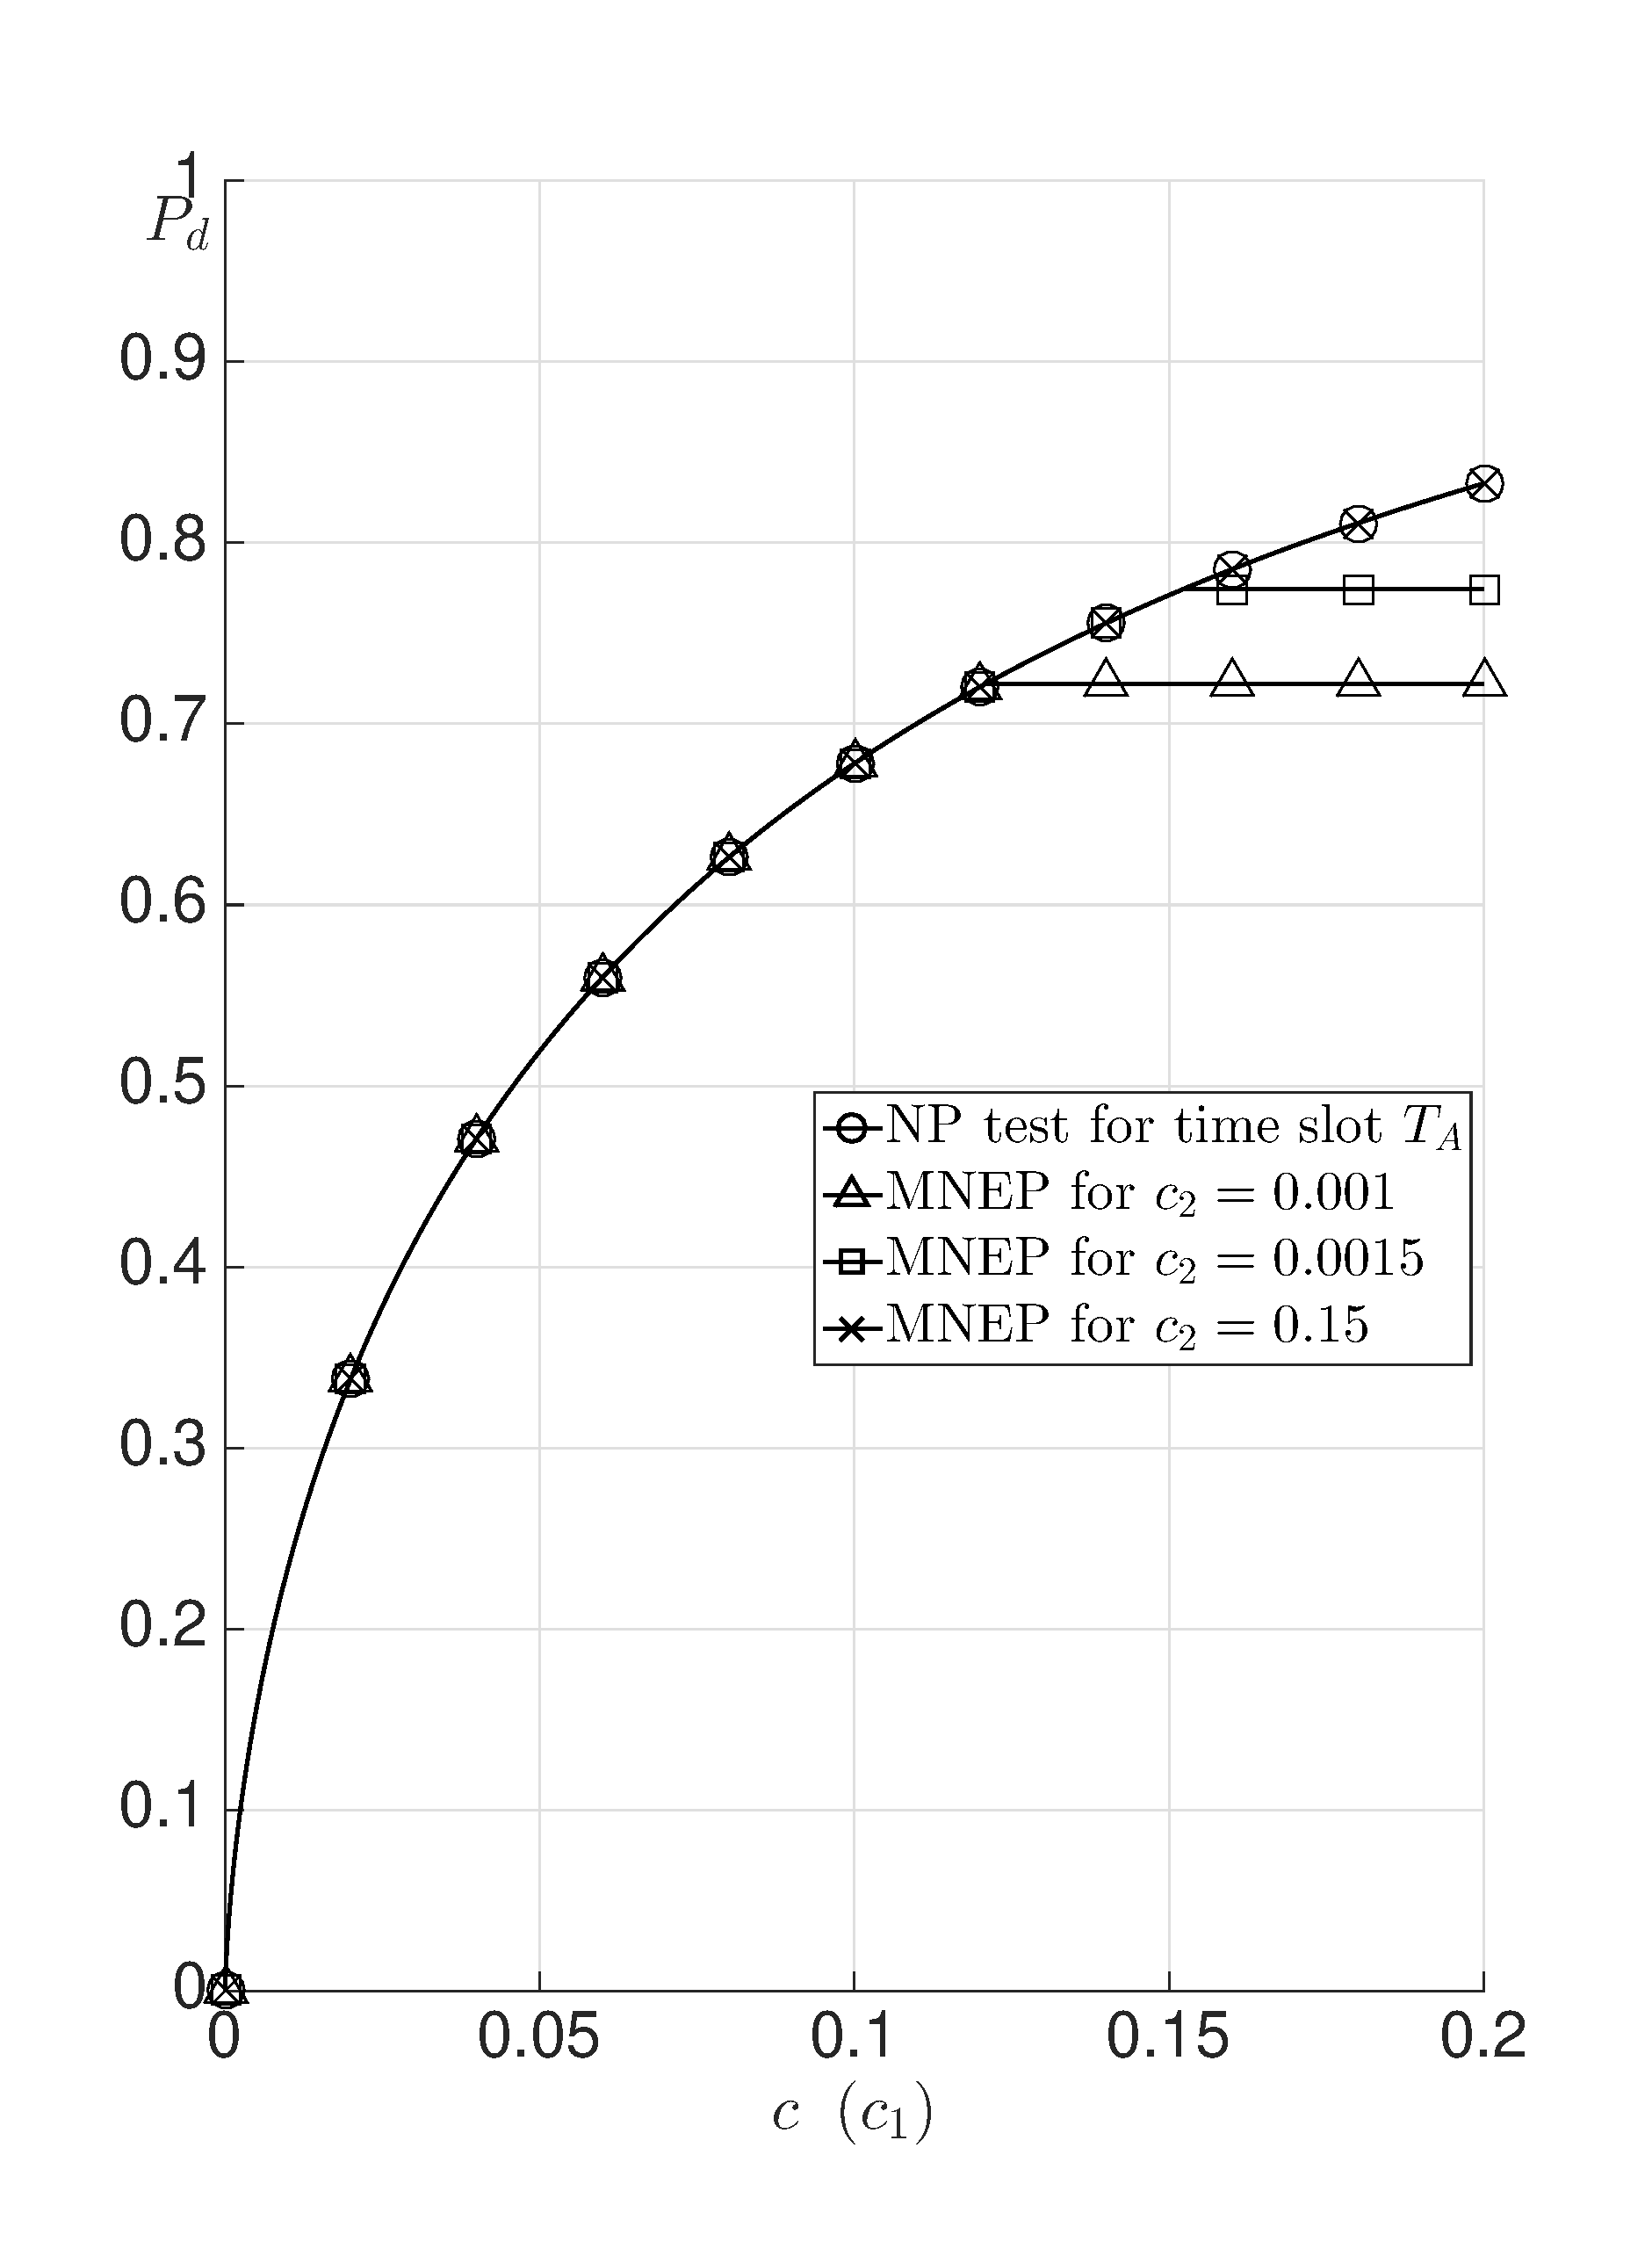
\includegraphics[width = 12cm]{5/SIa.eps}
  \caption{A comparison between the NP test and MENP test during time slot $T_A$.} 
  \label{pic:20150702a0}
\end{figure} 

During Time slot $T_A$, only primary signal $s_A$ could present in the channel. Under MENP framework, $P_{f_1}$ is the probability that the detector recognizes the channel is ideal while $s_A$ is transmitting. 
Hence under MENP framework, we consider the relationship between $P_d$ and $c_1$. The performance of MENP test is also illustrated in Figure \ref{pic:20150702a0}.  

As we can observe, with $c_2$  fixed to $0.001$ (or $0.0015$), when $c_1$ is smaller than $0.12$ (or $0.15$) the performance of MENP test and NP test are the same; when $c_1$ is larger than $0.12$ (or $0.15$) the NP test has better performance. This is reasonable.  
For both MENP test and the NP test with perfect side information, the decision rule can be written in form of
\begin{equation}
  y  \substack{\bar{H}_0 \\ \geq \\ < \\ H_0} V_\tau
\end{equation}
and the probability of detection is 
\begin{equation}
  P_d = F_0(V_\tau)\,.
\end{equation}
The above equation suggests $P_d$ is an increasing function with $V_\tau$. 
In the MENP test, $V_\tau$ is determined by $V_{\tau MENP}= \min (F_1^{-1}(c_1), F_2^{-1}(c_2))$; in the NP test with perfect side information, during time slot $T_A$, $V_\tau$ is determined by $V_{\tau NP A} = F_1^{-1}(c)$. When $c_1 \leq F_1(F_2^{-1}(c_2))$, i.e. $F_1^{-1}(c_1) \leq  F_2^{-1}(c_2)$, we have  $V_{\tau MENP} = F_1^{-1}(c_1)$. Since $V_{\tau NP A} = F_1^{-1}(c)$, when $c = c_1$, we have $V_{\tau MENP} = V_{\tau NPA}$, i.e.  $P_d(\delta_M) = P_d(\delta_{NP})$.    
When $c_1 > F_1(F_2^{-1}(c_2))$, i.e. $F_1^{-1}(c_1) > F_2^{-1}(c_2)$, we have  $V_{\tau MENP} = F_2^{-1}(c_2) < F_1^{-1}(c_1)$. Since $V_{\tau NP A} = F_1^{-1}(c)$, when $c = c_1$, we have 
$V_{\tau MENP} < V_{\tau NP}$, i.e.  $P_d(\delta_M) < P_d(\delta_{NP})$.
Hence for MENP test, with $c_2$ fixed, when $c_1$ is smaller than $F_1( F_2^{-1}(c_2) ) $, $P_d(\delta_M) = P_d(\delta_{NP})$; when $c_1$ is larger than $ F_1( F_2^{-1}(c_2))$, $P_d(\delta_M) < P_d(\delta_{NP})$. 
However for the situation when  $c_2$ is fixed to $0.15$, for $c_1 \in [0, 0.2]$, $c_1 <  F_1(F_2^{-1}(c_2))$ is always holds. Hence for the situation when $c_2$ is fixed to $0.15$ and $c_1 = c \leq 0.2$, the performance of MENP test and NP test are the same. This is verified in Figure \ref{pic:20150702a0}. 

Next we consider the performance of NP test and MENP test during time slot $T_B$.
The performance of NP test and MNEP test are shown in Figure \ref{pic:20150704a0}. During time slot $T_B$, only primary user $s_B$ could present in the channel. Under MENP framework, $P_{f_2}$ is the probability that the detector recognizes the channel is ideal while $s_B$ is transmitting. Hence under MENP framework, we consider the relationship between $P_d$ and $c_2$.

\begin{figure}[!hbp]
  \centering
  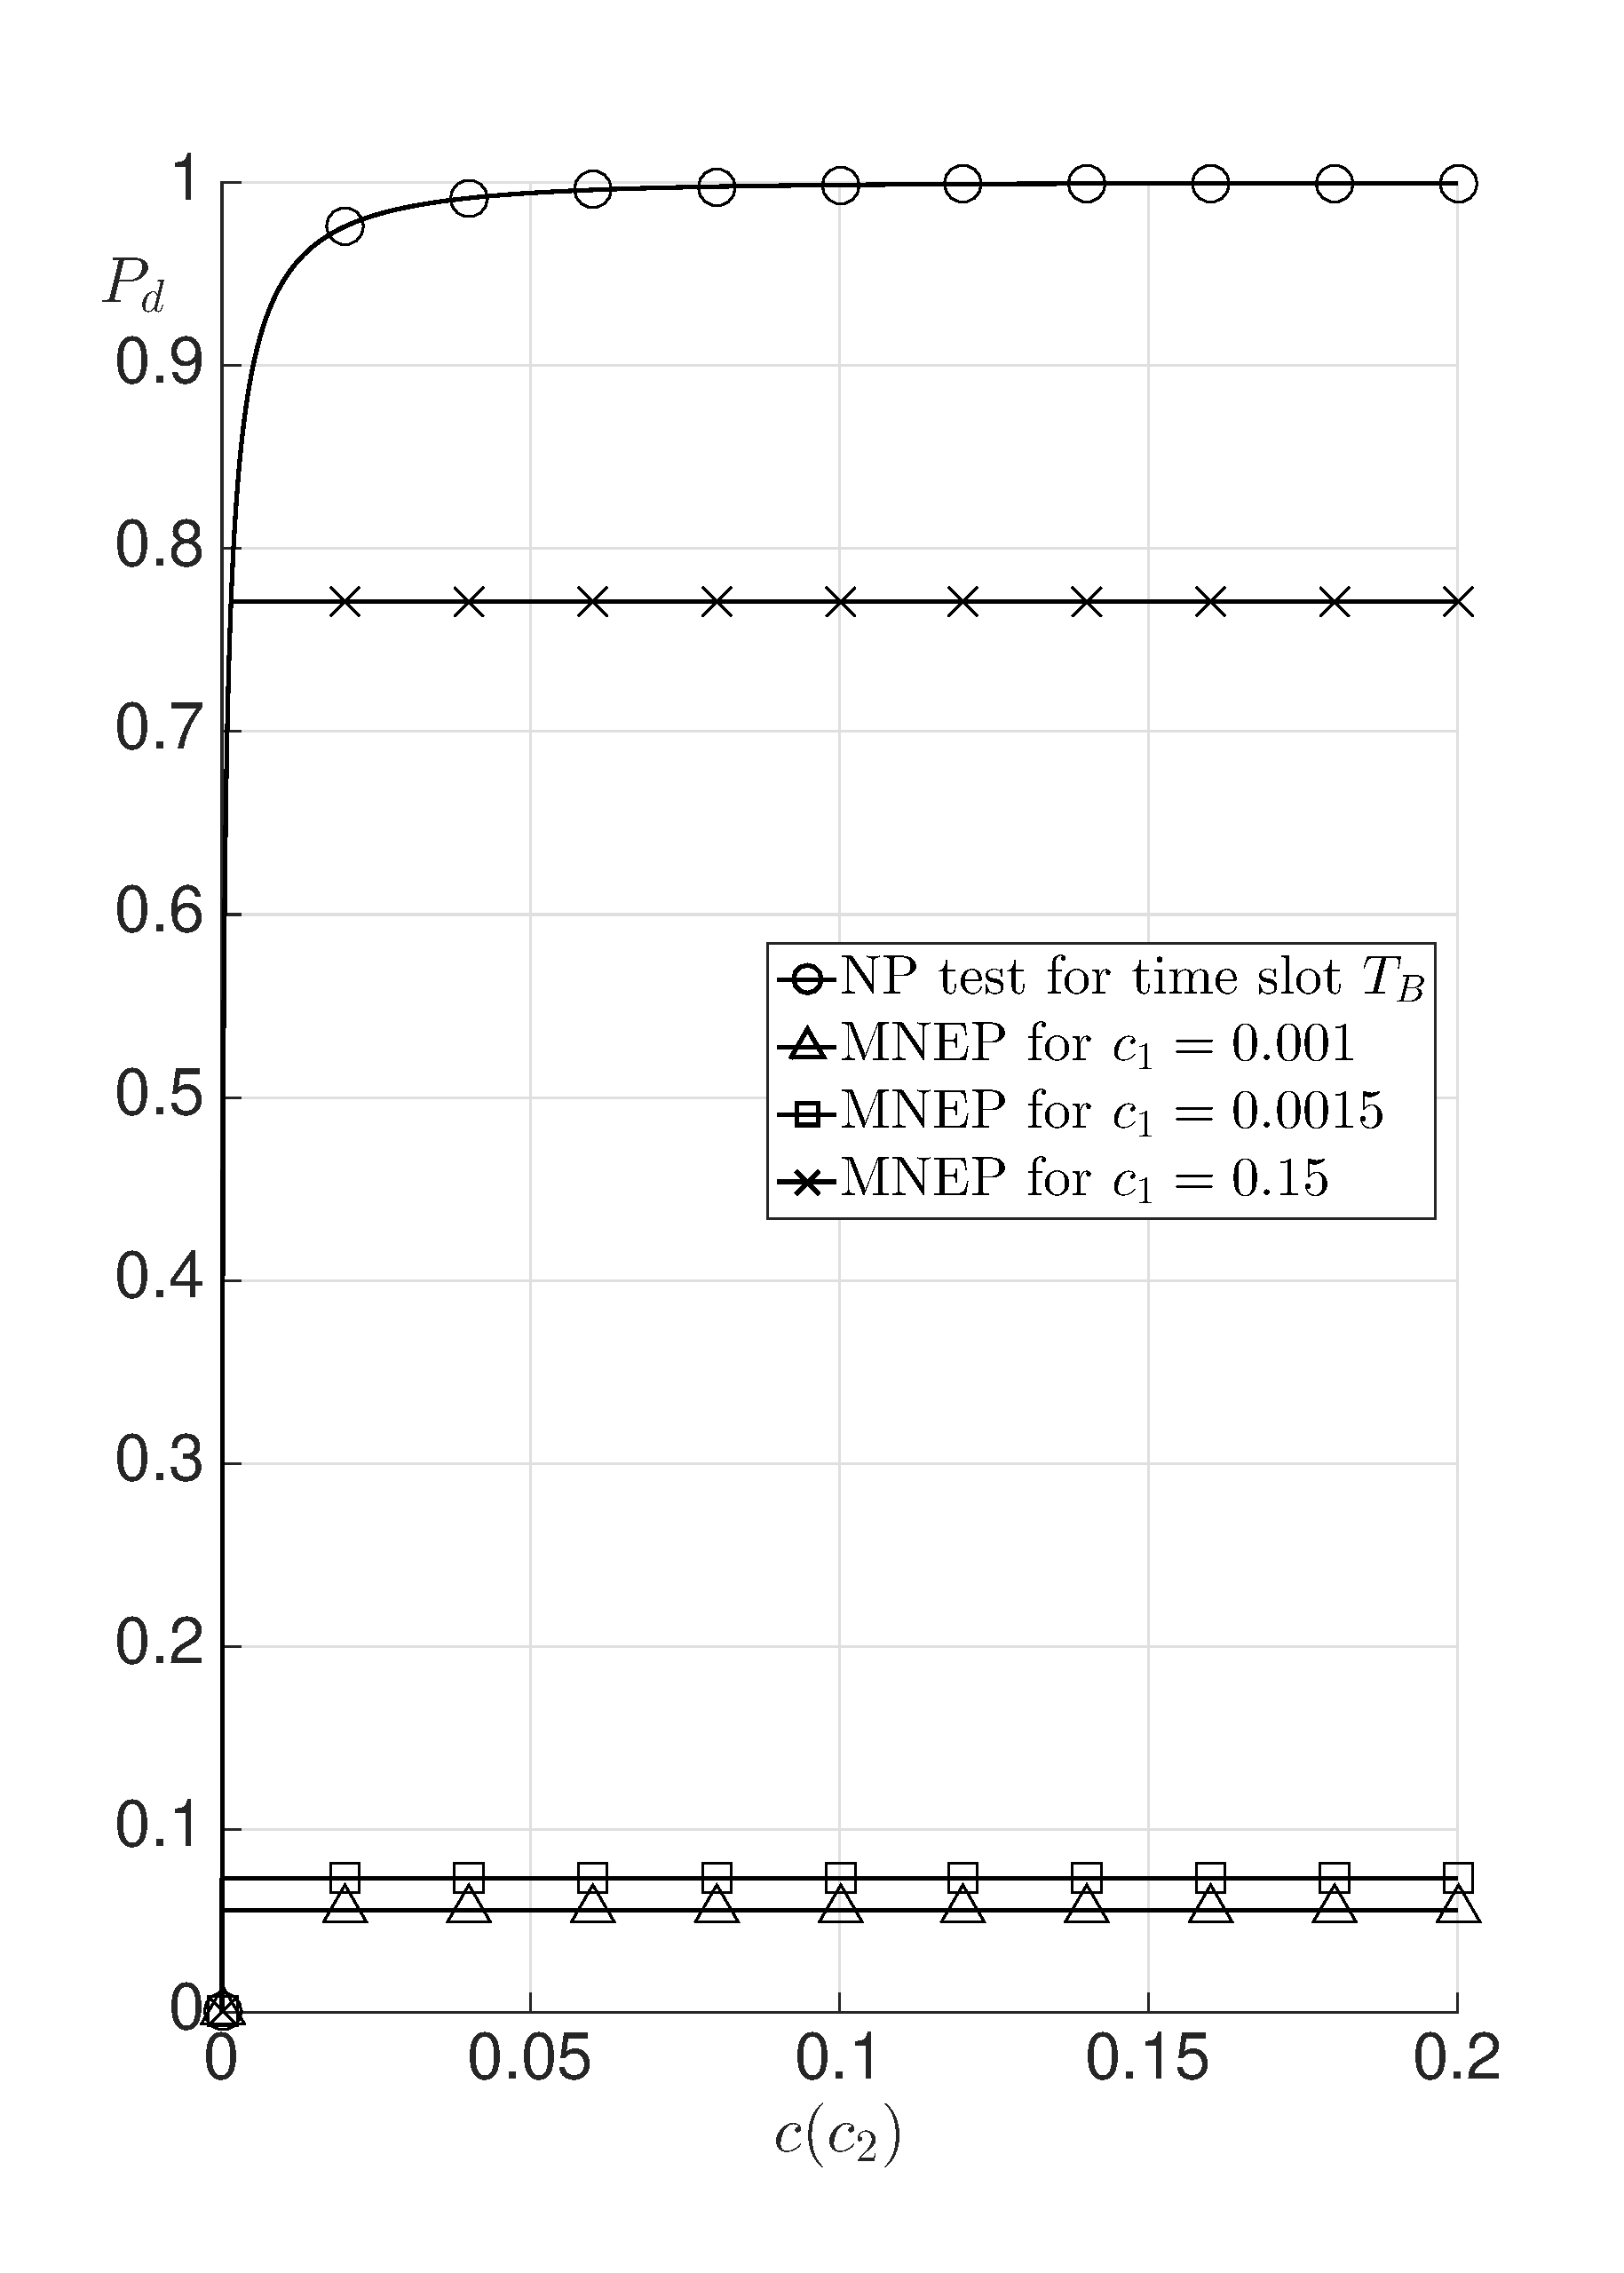
\includegraphics[width = 12cm]{5/SIb.eps}
  \caption{A comparison between the NP test and MENP test during time slot $T_B$.} 
  \label{pic:20150704a0}
\end{figure} 

As we can observe, with $c_1$  fixed, when $c_2$ is small the performance of MENP test and NP test are the same; when $c_2$ becomes larger the NP test has better performance. This is reasonable. In the MENP test, $V_\tau$ is determined by $V_{\tau MENP}= \min (F_1^{-1}(c_1), F_2^{-1}(c_2))$; in the NP test with perfect side information, during time slot $T_B$, $V_\tau$ is determined by $V_{\tau NP B} = F_2^{-1}(c)$. When $c_2 \leq F_2(F_1^{-1}(c_1))$, i.e. $F_1^{-1}(c_1) \geq  F_2^{-1}(c_2)$, we have  $V_{\tau MENP} = F_2^{-1}(c_2)$. Since $V_{\tau NP B} = F_2^{-1}(c)$, when $c = c_2$, we have $V_{\tau MENP} = V_{\tau NP B}$, i.e. $P_d(\delta_M) = P_d(\delta_{NP})$.    
When $c_2 > F_1(F_2^{-1}(c_1))$, i.e. $F_1^{-1}(c_1) < F_2^{-1}(c_2)$, we have  $V_{\tau MENP} = F_1^{-1}(c_1) < F_2^{-1}(c_2)$. Since $V_{\tau NP B} = F_2^{-1}(c)$, when $c = c_2$, we have  $V_{\tau MENP} < V_{\tau NP B}$, i.e.  $P_d(\delta_M) < P_d(\delta_{NP})$.
Hence for MENP test, with $c_1$ fixed, when $c_2$ is smaller than $ F_2( F_1^{-1}(c_1)) $, $P_d(\delta_M) = P_d(\delta_{NP})$; when $c_2$ is larger than $ F_2( F_1^{-1}(c_1)) $, $P_d(\delta_M) < P_d(\delta_{NP})$. 


